\section{Packed Hilbert R-tree}
\label{sec:rtree}
A Packed Hilbert R-tree is an extension of the R-tree, a balanced tree used for multidimensional data, in our case, spatial data. From \cite{rtree}, a regular R-tree stores all data as leaf nodes on the same level. All leaves have minimum bounding rectangles (MBRs) that geometrically contain the data element of that node. Parent nodes also have MBRs, MBRs of parents geoemtrically conatin all MBRs of the children. An example of this is shown in figure \ref{fig:rtree}, with the corresponding data in figure \ref{fig:mbrs}. This allows for efficient spatial queries. When querying with a spatial filter, the system will only explore nodes that have MBRs overlapping with the spatial filter. For large datasets, this can lead to significant performance gains for many queries, as much fewer nodes need to be accessed.

\begin{figure}
    \centering
    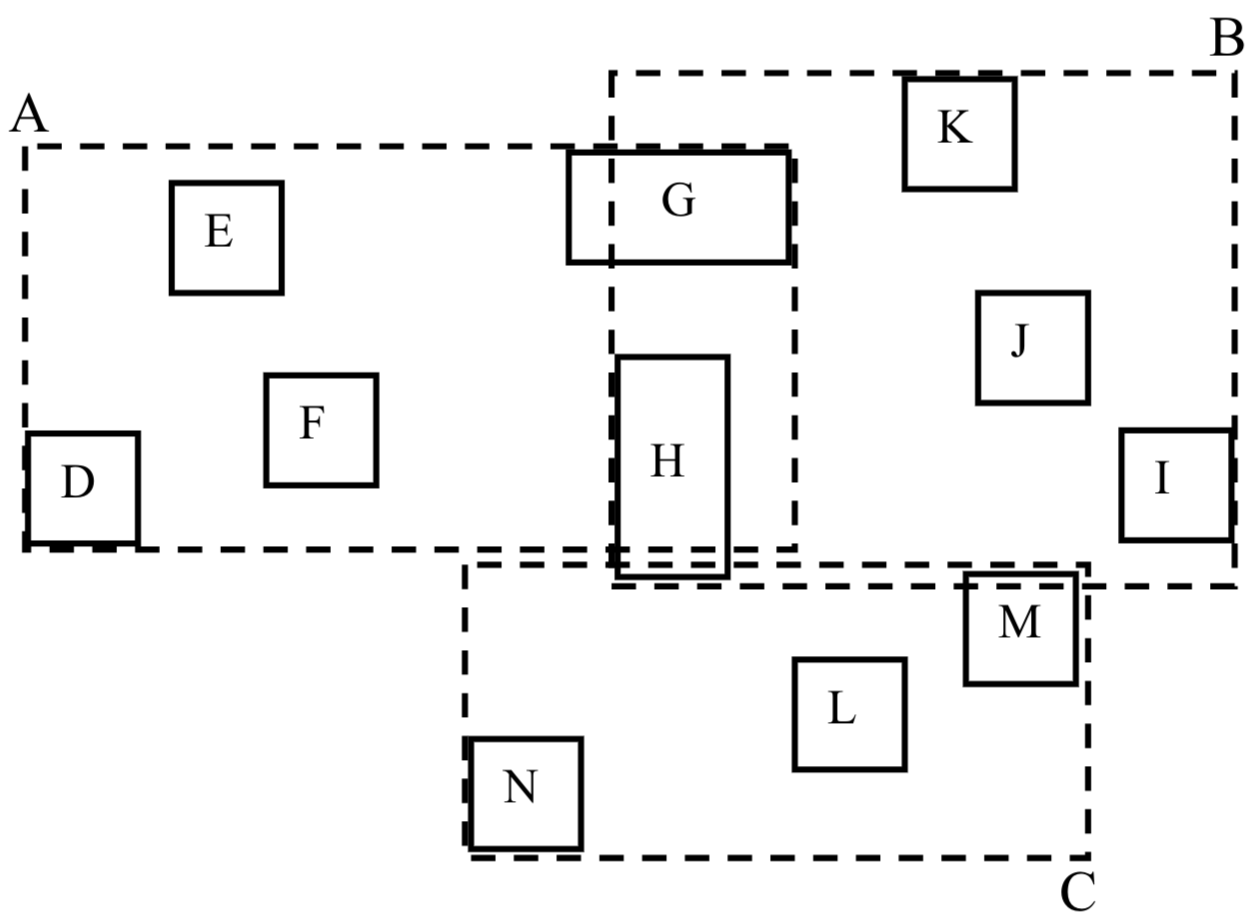
\includegraphics[width=0.5\linewidth]{./figures/mbrs.png}
    \caption{An example of data MBRs and their MBRs, from \cite{rtree}.}
    \label{fig:mbrs}
\end{figure}
\begin{figure}
    \centering
    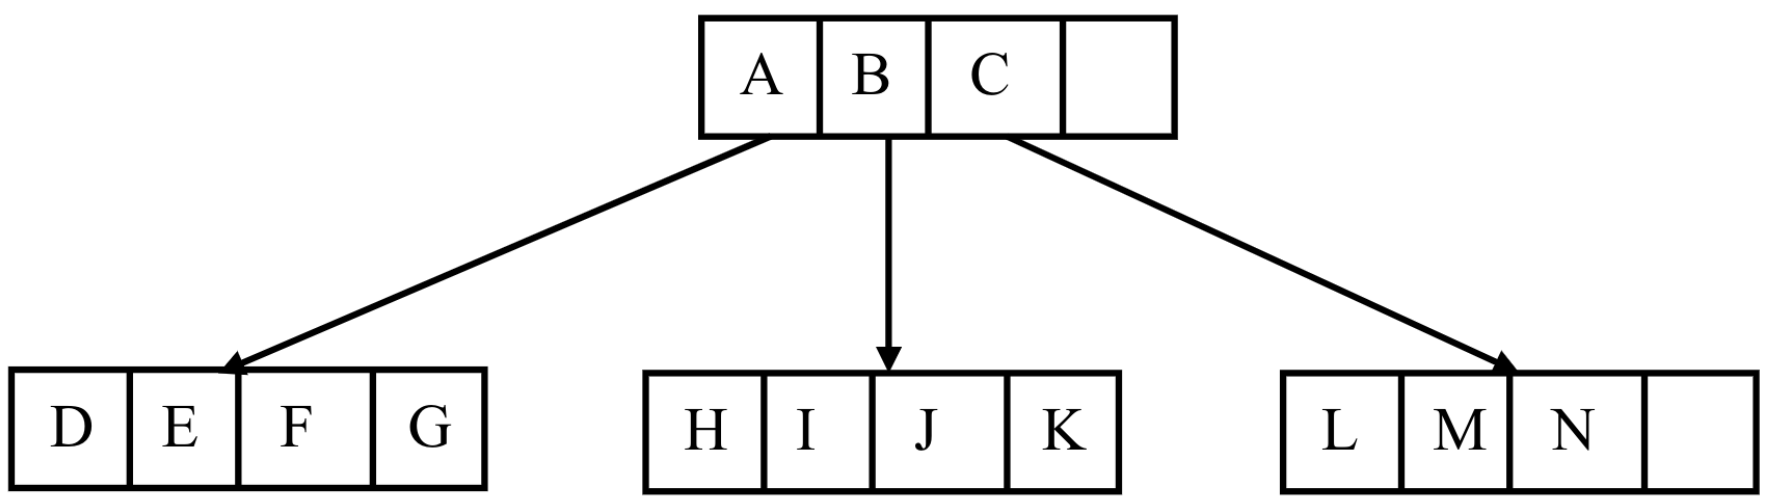
\includegraphics[width=\linewidth]{./figures/rtree.png}
    \caption{The corresponding R-tree, from \cite{rtree}.}
    \label{fig:rtree}
\end{figure}

What distinguishes a normal R-tree from a Hilbert R-tree is the MBR selection. The Hilbert R-tree utilizes Hilbert curves to generate MBRs for nodes. A Hilbert curve is a space-filling curve that can traverse every point in higher-dimensional space. This property allows for the mapping of two-dimensional values to one-dimensional values by drawing the curve in two dimensions and assigning ascending values to the points along the curve, see figure \ref{fig:hilbert} for Hilbert curves with corresponding values. These values are referred to as Hilbert values. Hilbert curves have the characteristic such that elements close in space will also be close in Hilbert values. By sorting MBRs based on the Hilbert value of the rectangle centroids, we can create MBRs with minimal overlap for spatial indexing.

\begin{figure}[t]
    \centering
    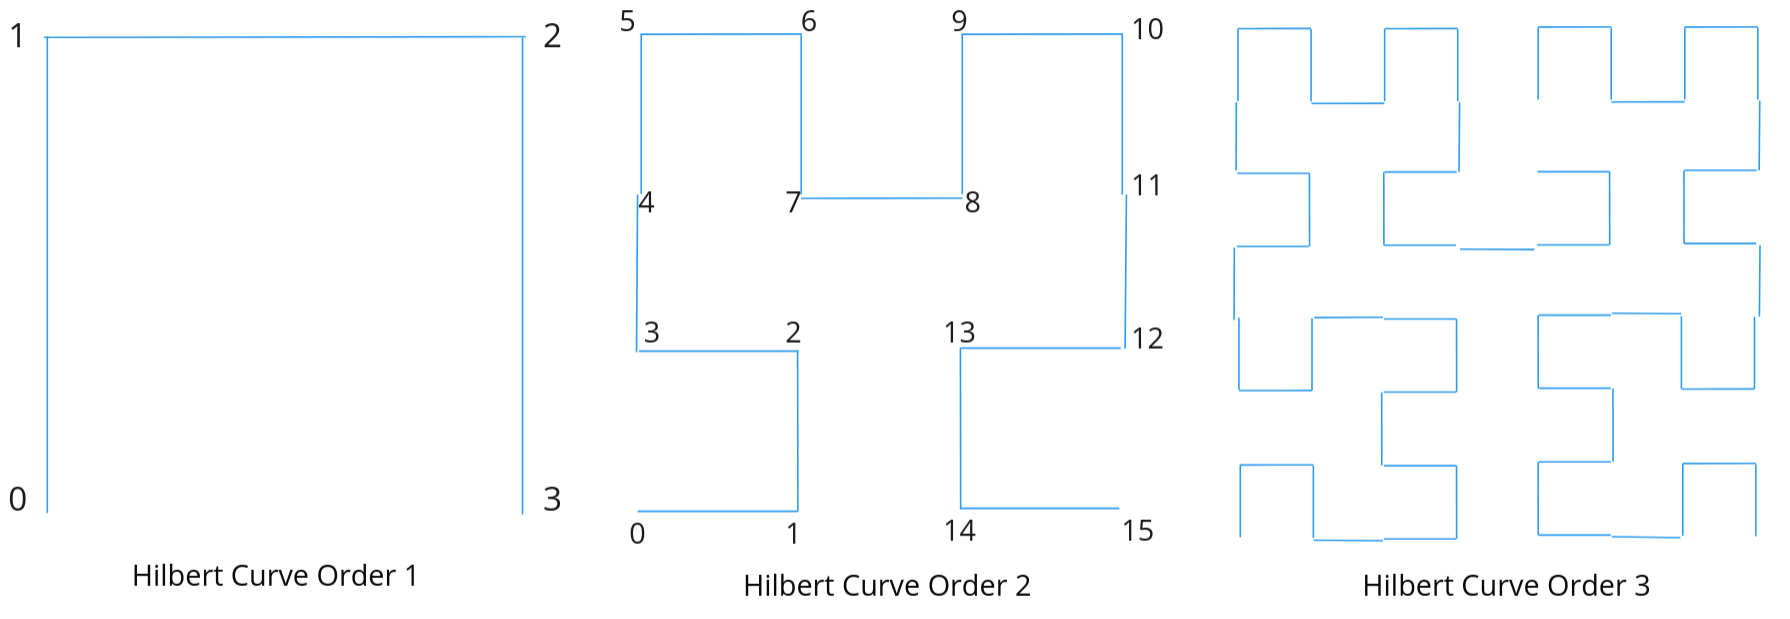
\includegraphics[width=\linewidth]{./figures/hilbert_orders.png}
    \caption{Showing Hilbert Curves of orders 1, 2, and 3.}
    \label{fig:hilbert}
\end{figure}

The Packed Hilbert R-tree is an optimized version of the Hilbert Tree. The Packed R-tree has even less overlap, resulting in improved query performance. The downside is that it requires more resources for construction. Considering the additional resource consumption, the Packed variant is only practical for applications that heavily prioritize read operations. In a system with frequent write operations, the entire tree would need to be rewritten frequently, leading to significant performance loss. For this reason, the Packed Hilbert R-tree is also known as the static Hilbert R-tree.